\let\negmedspace\undefined
\let\negthickspace\undefined
\documentclass[journal]{IEEEtran}
\usepackage[a5paper, margin=10mm, onecolumn]{geometry}
%\usepackage{lmodern} % Ensure lmodern is loaded for pdflatex
\usepackage{tfrupee} % Include tfrupee package

\setlength{\headheight}{1cm} % Set the height of the header box
\setlength{\headsep}{0mm}     % Set the distance between the header box and the top of the text

\usepackage{gvv-book}
\usepackage{gvv}
\usepackage{cite}
\usepackage{amsmath,amssymb,amsfonts,amsthm}
\usepackage{algorithmic}
\usepackage{graphicx}
\usepackage{textcomp}
\usepackage{xcolor}
\usepackage{txfonts}
\usepackage{listings}
\usepackage{enumitem}
\usepackage{mathtools}
\usepackage{gensymb}
\usepackage{comment}
\usepackage[breaklinks=true]{hyperref}
\usepackage{tkz-euclide} 
\usepackage{listings}
\usepackage{gvv}                                        
\def\inputGnumericTable{}                                 
\usepackage[latin1]{inputenc}                                
\usepackage{color}                                            
\usepackage{array}                                            
\usepackage{longtable}                                       
\usepackage{calc}                                             
\usepackage{multirow}                                         
\usepackage{hhline}                                           
\usepackage{ifthen}                                           
\usepackage{lscape}
\begin{document}

\bibliographystyle{IEEEtran}
\vspace{3cm}

\title{4.4.9}
\author{AI24BTECH11024-Pappuri Prahladha}
% \bigskip
{\let\newpage\relax\maketitle}

\renewcommand{\thefigure}{\theenumi}
\renewcommand{\thetable}{\theenumi}
\setlength{\intextsep}{10pt} % Space between text and floats


\numberwithin{equation}{enumi}
\numberwithin{figure}{enumi}
\renewcommand{\thetable}{\theenumi}


\textbf{Question:}\\
The vector equation of the line 
\begin{align*}
	\frac{x-5}{3}=\frac{y+4}{7}=\frac{z-6}{2} 
\end{align*}
is \noindent\rule{1cm}{0.1pt}.\\
\\
\textbf{Solution: }\\
\begin{table}[h!]
    \renewcommand{\thetable}{1}
    \centering
    \begin{tabular}[12ptx]{ |c| c|}
\hline\textbf{Term} & \textbf{Description}\\
\hline
$\hat{i}$ and $-\hat{i}$ & Unit vectors along East and West directions \\

\hline
$\hat{j}$ and -$\hat{j}$ & Unit vectors along North and south directions\\
\hline
$\vec{V_{1}}$ or Vector 1 and $\vec{V_{2}}$ or Vector 2 & velocity vectors of Rain and Wind\\
\hline
$\vec{V_{3}}$ or Vector 3 & Resultant velocity vector of Rain and Wind\\
\hline
$\theta$ & Required angle with the horizontal\\
\hline
\end{tabular}
    \caption{Terms used}
    \label{TABLE 1:}
\end{table}\\
The given line is passing through: \\
\begin{align*}
\vec{A}=\begin{pmatrix}
5\\
-4\\
6
\end{pmatrix},
\vec{B}=\begin{pmatrix}
8\\
3\\
8
\end{pmatrix},
\vec{C}=\begin{pmatrix}
2\\
-11\\
4
\end{pmatrix}   
\end{align*}\\
 From equation \eqref{dir-vec} ,the direction vector of the line is\\
\begin{align}
\vec{m}=\vec{B}-\vec{C}=\begin{pmatrix}
3\\
7\\
2
\end{pmatrix}  
\end{align}\\
from equation \eqref{eq:param-form}, the vector equation of line is passing through $\vec{A}$ and having direction vector $\vec{m}$ given by,\\
\begin{equation}
    \vec{x}=\vec{A}+\kappa\vec{m}
\end{equation}
from  equation 0.2, the vector equation of the given line is,
\begin{equation*}
    \vec{x}=\begin{pmatrix}
        5\\
        -4\\
        6
    \end{pmatrix}+\kappa\begin{pmatrix}
        3\\
        7\\
        2
    \end{pmatrix}
\end{equation*}

 \begin{figure}[h!]
   \centering
   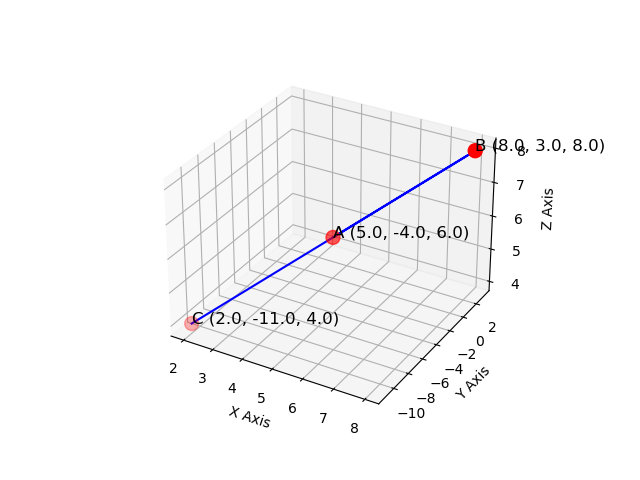
\includegraphics[width=0.7\linewidth]{figs/figure1.png}
   \caption{Plot showing the given line}
   \label{stemplot}
\end{figure}






\end{document}
